% Options for packages loaded elsewhere
\PassOptionsToPackage{unicode}{hyperref}
\PassOptionsToPackage{hyphens}{url}
%
\documentclass[
  8pt,
  ignorenonframetext,
]{beamer}
\author{}
\date{\vspace{-2.5em}}

\usepackage{pgfpages}
\setbeamertemplate{caption}[numbered]
\setbeamertemplate{caption label separator}{: }
\setbeamercolor{caption name}{fg=normal text.fg}
\beamertemplatenavigationsymbolsempty
% Prevent slide breaks in the middle of a paragraph
\widowpenalties 1 10000
\raggedbottom
\setbeamertemplate{part page}{
  \centering
  \begin{beamercolorbox}[sep=16pt,center]{part title}
    \usebeamerfont{part title}\insertpart\par
  \end{beamercolorbox}
}
\setbeamertemplate{section page}{
  \centering
  \begin{beamercolorbox}[sep=12pt,center]{part title}
    \usebeamerfont{section title}\insertsection\par
  \end{beamercolorbox}
}
\setbeamertemplate{subsection page}{
  \centering
  \begin{beamercolorbox}[sep=8pt,center]{part title}
    \usebeamerfont{subsection title}\insertsubsection\par
  \end{beamercolorbox}
}
\AtBeginPart{
  \frame{\partpage}
}
\AtBeginSection{
  \ifbibliography
  \else
    \frame{\sectionpage}
  \fi
}
\AtBeginSubsection{
  \frame{\subsectionpage}
}
\usepackage{amsmath,amssymb}
\usepackage{lmodern}
\usepackage{iftex}
\ifPDFTeX
  \usepackage[T1]{fontenc}
  \usepackage[utf8]{inputenc}
  \usepackage{textcomp} % provide euro and other symbols
\else % if luatex or xetex
  \usepackage{unicode-math}
  \defaultfontfeatures{Scale=MatchLowercase}
  \defaultfontfeatures[\rmfamily]{Ligatures=TeX,Scale=1}
\fi
% Use upquote if available, for straight quotes in verbatim environments
\IfFileExists{upquote.sty}{\usepackage{upquote}}{}
\IfFileExists{microtype.sty}{% use microtype if available
  \usepackage[]{microtype}
  \UseMicrotypeSet[protrusion]{basicmath} % disable protrusion for tt fonts
}{}
\makeatletter
\@ifundefined{KOMAClassName}{% if non-KOMA class
  \IfFileExists{parskip.sty}{%
    \usepackage{parskip}
  }{% else
    \setlength{\parindent}{0pt}
    \setlength{\parskip}{6pt plus 2pt minus 1pt}}
}{% if KOMA class
  \KOMAoptions{parskip=half}}
\makeatother
\usepackage{xcolor}
\IfFileExists{xurl.sty}{\usepackage{xurl}}{} % add URL line breaks if available
\IfFileExists{bookmark.sty}{\usepackage{bookmark}}{\usepackage{hyperref}}
\hypersetup{
  hidelinks,
  pdfcreator={LaTeX via pandoc}}
\urlstyle{same} % disable monospaced font for URLs
\newif\ifbibliography
\usepackage{color}
\usepackage{fancyvrb}
\newcommand{\VerbBar}{|}
\newcommand{\VERB}{\Verb[commandchars=\\\{\}]}
\DefineVerbatimEnvironment{Highlighting}{Verbatim}{commandchars=\\\{\}}
% Add ',fontsize=\small' for more characters per line
\usepackage{framed}
\definecolor{shadecolor}{RGB}{248,248,248}
\newenvironment{Shaded}{\begin{snugshade}}{\end{snugshade}}
\newcommand{\AlertTok}[1]{\textcolor[rgb]{0.94,0.16,0.16}{#1}}
\newcommand{\AnnotationTok}[1]{\textcolor[rgb]{0.56,0.35,0.01}{\textbf{\textit{#1}}}}
\newcommand{\AttributeTok}[1]{\textcolor[rgb]{0.77,0.63,0.00}{#1}}
\newcommand{\BaseNTok}[1]{\textcolor[rgb]{0.00,0.00,0.81}{#1}}
\newcommand{\BuiltInTok}[1]{#1}
\newcommand{\CharTok}[1]{\textcolor[rgb]{0.31,0.60,0.02}{#1}}
\newcommand{\CommentTok}[1]{\textcolor[rgb]{0.56,0.35,0.01}{\textit{#1}}}
\newcommand{\CommentVarTok}[1]{\textcolor[rgb]{0.56,0.35,0.01}{\textbf{\textit{#1}}}}
\newcommand{\ConstantTok}[1]{\textcolor[rgb]{0.00,0.00,0.00}{#1}}
\newcommand{\ControlFlowTok}[1]{\textcolor[rgb]{0.13,0.29,0.53}{\textbf{#1}}}
\newcommand{\DataTypeTok}[1]{\textcolor[rgb]{0.13,0.29,0.53}{#1}}
\newcommand{\DecValTok}[1]{\textcolor[rgb]{0.00,0.00,0.81}{#1}}
\newcommand{\DocumentationTok}[1]{\textcolor[rgb]{0.56,0.35,0.01}{\textbf{\textit{#1}}}}
\newcommand{\ErrorTok}[1]{\textcolor[rgb]{0.64,0.00,0.00}{\textbf{#1}}}
\newcommand{\ExtensionTok}[1]{#1}
\newcommand{\FloatTok}[1]{\textcolor[rgb]{0.00,0.00,0.81}{#1}}
\newcommand{\FunctionTok}[1]{\textcolor[rgb]{0.00,0.00,0.00}{#1}}
\newcommand{\ImportTok}[1]{#1}
\newcommand{\InformationTok}[1]{\textcolor[rgb]{0.56,0.35,0.01}{\textbf{\textit{#1}}}}
\newcommand{\KeywordTok}[1]{\textcolor[rgb]{0.13,0.29,0.53}{\textbf{#1}}}
\newcommand{\NormalTok}[1]{#1}
\newcommand{\OperatorTok}[1]{\textcolor[rgb]{0.81,0.36,0.00}{\textbf{#1}}}
\newcommand{\OtherTok}[1]{\textcolor[rgb]{0.56,0.35,0.01}{#1}}
\newcommand{\PreprocessorTok}[1]{\textcolor[rgb]{0.56,0.35,0.01}{\textit{#1}}}
\newcommand{\RegionMarkerTok}[1]{#1}
\newcommand{\SpecialCharTok}[1]{\textcolor[rgb]{0.00,0.00,0.00}{#1}}
\newcommand{\SpecialStringTok}[1]{\textcolor[rgb]{0.31,0.60,0.02}{#1}}
\newcommand{\StringTok}[1]{\textcolor[rgb]{0.31,0.60,0.02}{#1}}
\newcommand{\VariableTok}[1]{\textcolor[rgb]{0.00,0.00,0.00}{#1}}
\newcommand{\VerbatimStringTok}[1]{\textcolor[rgb]{0.31,0.60,0.02}{#1}}
\newcommand{\WarningTok}[1]{\textcolor[rgb]{0.56,0.35,0.01}{\textbf{\textit{#1}}}}
\setlength{\emergencystretch}{3em} % prevent overfull lines
\providecommand{\tightlist}{%
  \setlength{\itemsep}{0pt}\setlength{\parskip}{0pt}}
\setcounter{secnumdepth}{-\maxdimen} % remove section numbering
\newlength{\cslhangindent}
\setlength{\cslhangindent}{1.5em}
\newlength{\csllabelwidth}
\setlength{\csllabelwidth}{3em}
\newlength{\cslentryspacingunit} % times entry-spacing
\setlength{\cslentryspacingunit}{\parskip}
\newenvironment{CSLReferences}[2] % #1 hanging-ident, #2 entry spacing
 {% don't indent paragraphs
  \setlength{\parindent}{0pt}
  % turn on hanging indent if param 1 is 1
  \ifodd #1
  \let\oldpar\par
  \def\par{\hangindent=\cslhangindent\oldpar}
  \fi
  % set entry spacing
  \setlength{\parskip}{#2\cslentryspacingunit}
 }%
 {}
\usepackage{calc}
\newcommand{\CSLBlock}[1]{#1\hfill\break}
\newcommand{\CSLLeftMargin}[1]{\parbox[t]{\csllabelwidth}{#1}}
\newcommand{\CSLRightInline}[1]{\parbox[t]{\linewidth - \csllabelwidth}{#1}\break}
\newcommand{\CSLIndent}[1]{\hspace{\cslhangindent}#1}
% type setting
% ------------------------------------------------------------------------------
\usepackage[german]{babel}     

% fonts
% ------------------------------------------------------------------------------
\usefonttheme{professionalfonts}

% slide title and horizontal line
% ------------------------------------------------------------------------------
\setbeamertemplate{frametitle}{%
    \vskip-30pt \color{black}\large%
    \begin{minipage}[b][23pt]{120mm}%
    \flushleft\insertframetitle%
    \end{minipage}%
}

\setbeamertemplate{headline}										
{
\vskip10pt\hfill\hspace{3.5mm} 										 
\vskip15pt\color{black}\rule{\textwidth}{0.4pt} 					 
}

% slide number
% ---------------------------------------------------------------
\setbeamertemplate{navigation symbols}{}
\setbeamertemplate{footline}
{
\vskip5pt
\vskip2pt
\makebox[123mm]{\hspace{7.5mm}
\hfill Allgemeines Lineares Modell $\vert$ 
\copyright $ $ 2022 Dirk Ostwald CC BY-NC-SA 4.0 $\vert$ 
Folie \insertframenumber}
\vskip4pt
}

% block color scheme
% ------------------------------------------------------------------------------
% colors
\definecolor{white}{RGB}{255,255,255}
\definecolor{grey}{RGB}{235,235,235}
\definecolor{lightgrey}{RGB}{245,245,245}
\definecolor{LightBlue}{RGB}{220,220,255}
\definecolor{darkblue}{RGB}{51, 51, 153}

% definitions and theorems
\setbeamercolor{block title}{fg = black, bg = grey}
\setbeamercolor{block body}{fg = black, bg = lightgrey}

% general line spacing 
% ------------------------------------------------------------------------------
\linespread{1.3}

% local line spacing
% ------------------------------------------------------------------------------
\usepackage{setspace}

% colors
% -----------------------------------------------------------------------------
\usepackage{color}

% justified text
% ------------------------------------------------------------------------------
\usepackage{ragged2e}
\usepackage{etoolbox}
\apptocmd{\frame}{}{\justifying}{}

% bullet point lists
% -----------------------------------------------------------------------------
\setbeamertemplate{itemize item}[circle]
\setbeamertemplate{itemize subitem}[circle]
\setbeamertemplate{itemize subsubitem}[circle]
\setbeamercolor{itemize item}{fg = black}
\setbeamercolor{itemize subitem}{fg = black}
\setbeamercolor{itemize subsubitem}{fg = black}
\setbeamercolor{enumerate item}{fg = black}
\setbeamercolor{enumerate subitem}{fg = black}
\setbeamercolor{enumerate subsubitem}{fg = black}
\setbeamerfont{itemize/enumerate body}{}
\setbeamerfont{itemize/enumerate subbody}{size = \normalsize}
\setbeamerfont{itemize/enumerate subsubbody}{size = \normalsize}

% color links
% ------------------------------------------------------------------------------
\usepackage{hyperref}
\definecolor{urls}{RGB}{204,0,0}
\hypersetup{colorlinks, citecolor = darkblue, urlcolor = urls}


% additional math commands
% ------------------------------------------------------------------------------
\usepackage{bm}                                         
\newcommand{\niton}{\not\owns}
\DeclareMathOperator*{\intinf}{\int_{-\infty}^{\infty}}


% text highlighting
% ------------------------------------------------------------------------------
\usepackage{soul}
\makeatletter
\let\HL\hl
\renewcommand\hl{%
  \let\set@color\beamerorig@set@color
  \let\reset@color\beamerorig@reset@color
  \HL}
\makeatother

% equation highlighting
% -----------------------------------------------------------------------------
\newcommand{\highlight}[2][yellow]{\mathchoice%
  {\colorbox{#1}{$\displaystyle#2$}}%
  {\colorbox{#1}{$\textstyle#2$}}%
  {\colorbox{#1}{$\scriptstyle#2$}}%
  {\colorbox{#1}{$\scriptscriptstyle#2$}}}%

% additional mathematical operators
% ------------------------------------------------------------------------------
\DeclareMathOperator*{\argmax}{arg\,max}
\DeclareMathOperator*{\argmin}{arg\,min}

\ifLuaTeX
  \usepackage{selnolig}  % disable illegal ligatures
\fi

\begin{document}

\begin{frame}[plain]{}
\protect\hypertarget{section}{}
\center

\begin{center}
\includegraphics[width=0.2\linewidth]{6_Abbildungen/alm_6_otto} \end{center}

\vspace{2mm}

\huge

Allgemeines Lineares Modell \vspace{6mm}

\large

BSc Psychologie SoSe 2022

\vspace{6mm}
\normalsize

Prof.~Dr.~Dirk Ostwald
\end{frame}

\begin{frame}[plain]{}
\protect\hypertarget{section-1}{}
\center
\huge
\vfill

\noindent (6) Modellschätzung \vfill
\end{frame}

\begin{frame}{Überblick}
\protect\hypertarget{uxfcberblick}{}
\large

Naturwissenschaft \vspace{7mm}

\begin{center}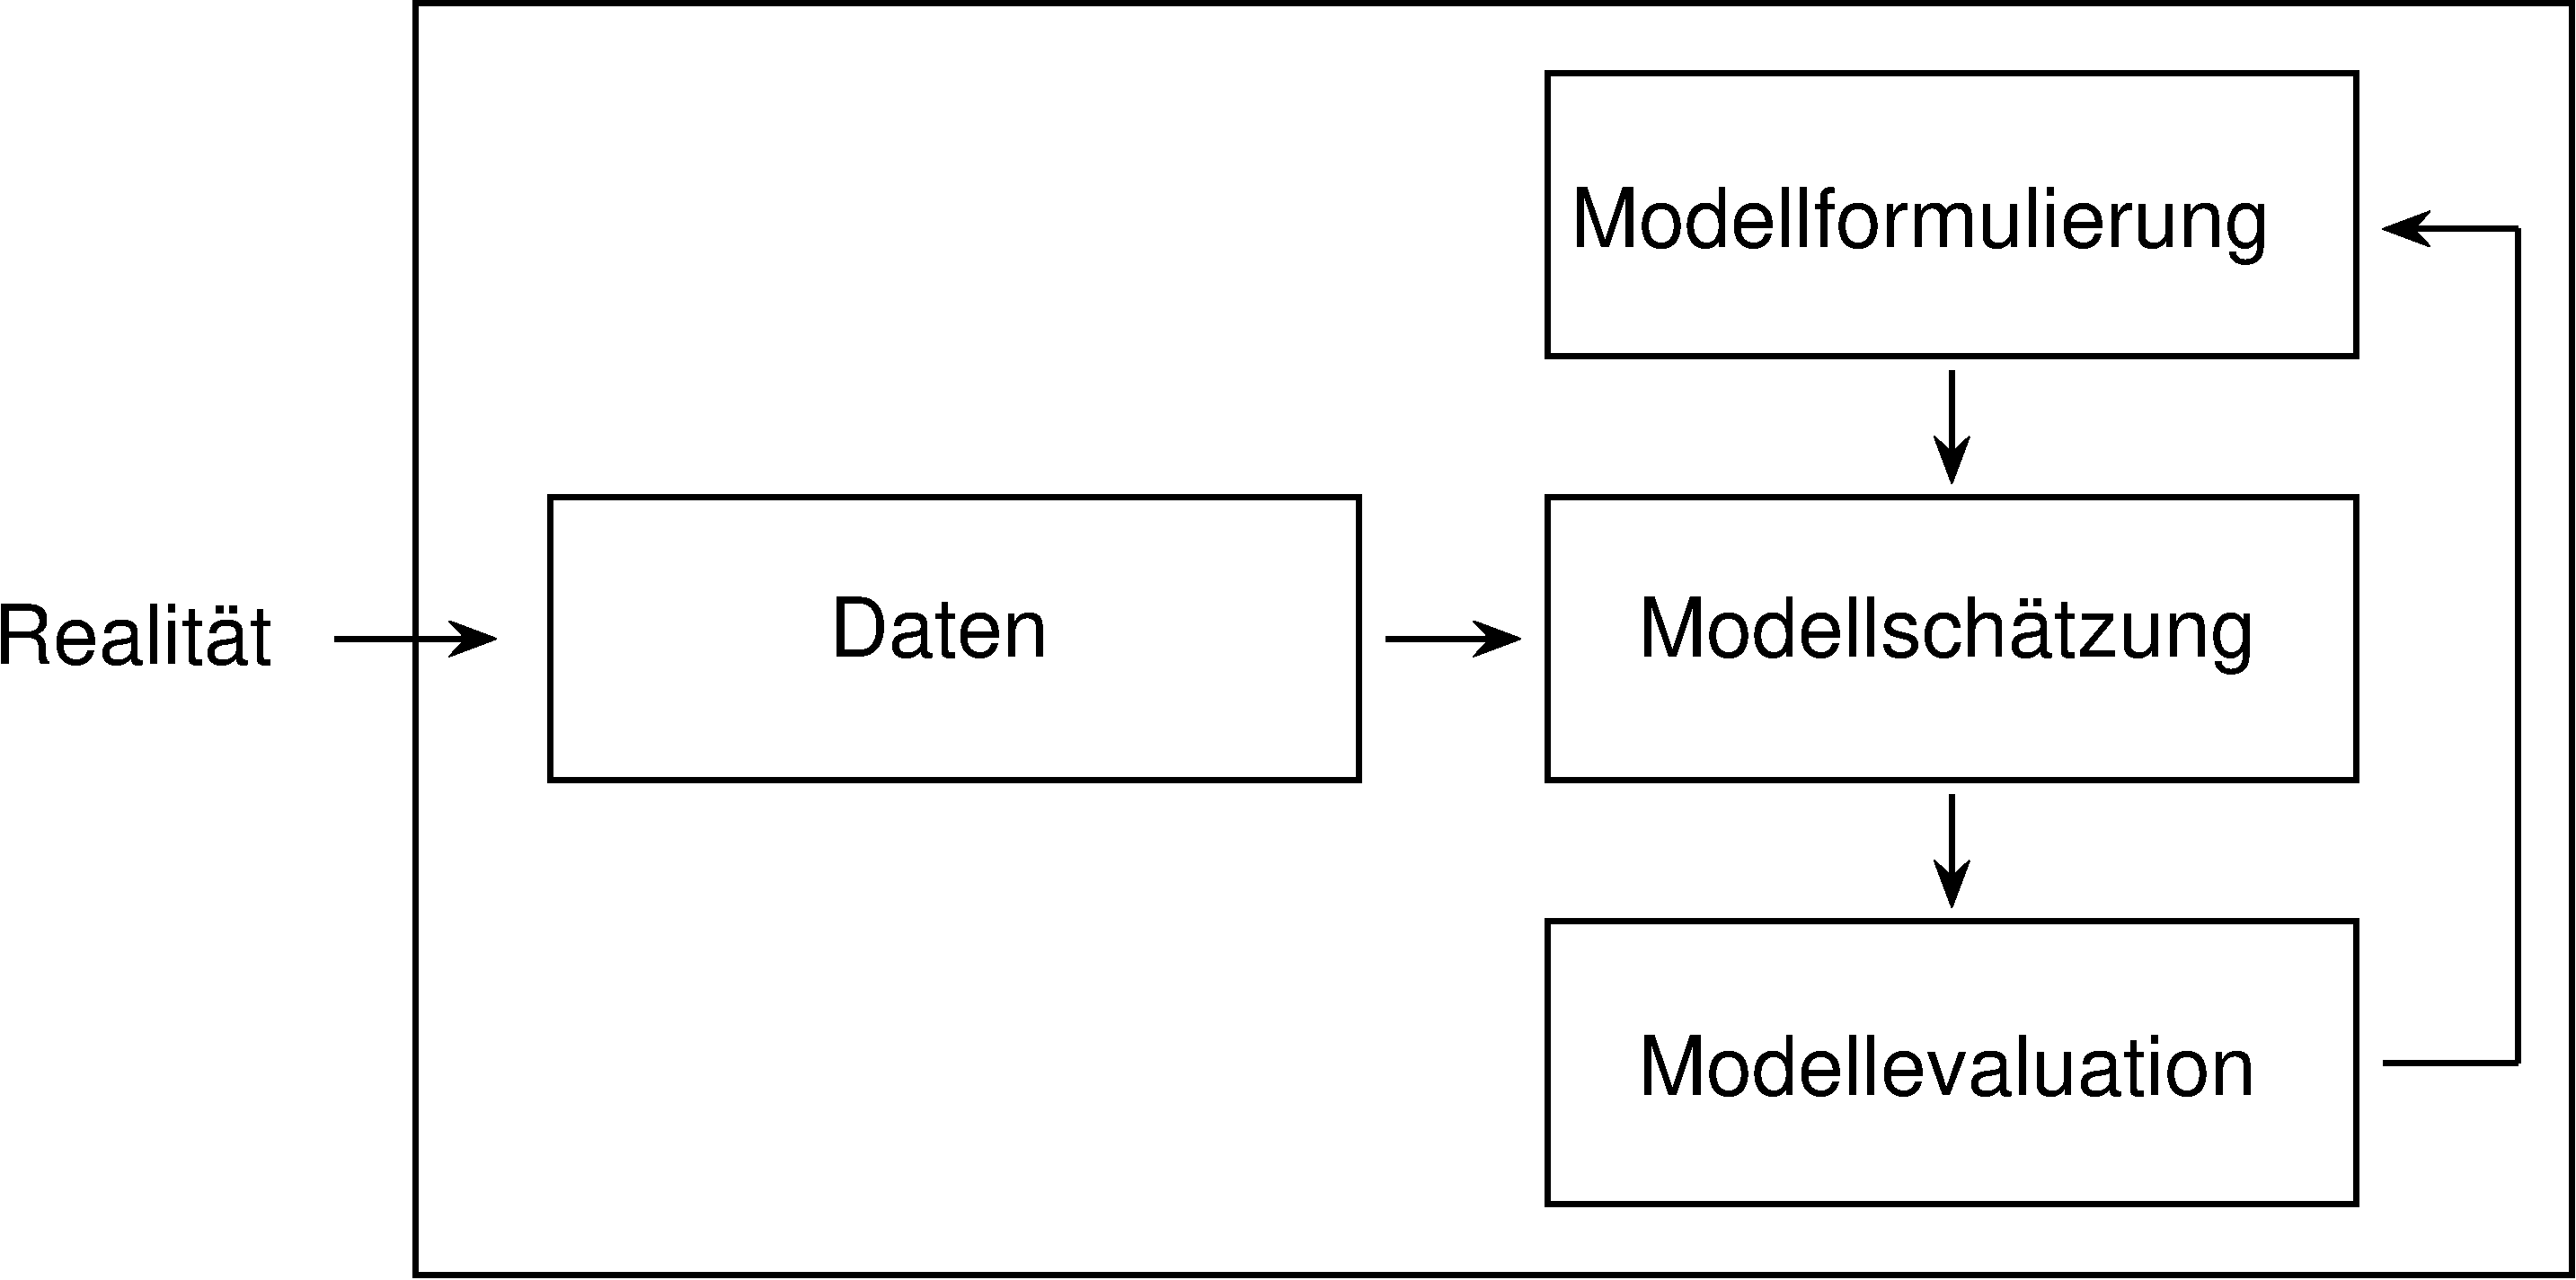
\includegraphics[width=0.9\linewidth]{6_Abbildungen/alm_6_wissenschaft} \end{center}
\end{frame}

\begin{frame}{Überblick}
\protect\hypertarget{uxfcberblick-1}{}
\vspace{1mm}
\normalsize

Modellformulierung \vspace{1mm} \small \begin{equation}
y = X\beta + \varepsilon, \varepsilon \sim N(0_n,\sigma^2I_n)
\end{equation} \vspace{5mm}

\normalsize

Modellschätzung \small \begin{equation}
\hat{\beta} = (X^TX)^{-1} X^Ty,  \hat{\sigma}^2 = \frac{(y - X\hat{\beta})^T(y - X\hat{\beta})}{n-p}
\end{equation} \vspace{4mm}

\normalsize

Modellevaluation \small \begin{equation}
T = \frac{c^T\hat{\beta} - c^T\beta_0}{\sqrt{\hat{\sigma}^2(X^TX)^{-1}c}}, 
F = \frac{(\hat{\varepsilon}_1^T\hat{\varepsilon}_1 - \hat{\varepsilon}^T\hat{\varepsilon})/p_2}{\hat{\varepsilon}^T\hat{\varepsilon}/(n-p)}
\end{equation}
\end{frame}

\begin{frame}{Überblick}
\protect\hypertarget{uxfcberblick-2}{}
Standardprobleme Frequentistischer Inferenz \small

\noindent (1) Parameterschätzung

Ziel der Parameterschätzung ist es, einen möglichst guten Tipp für die
wahren, aber unbekannten, Parameterwerte (oder eine Funktion derer)
abzugeben, typischerweise basierend auf der Beobachtung einer
Datenrealisierung. \vspace{2mm}

\noindent (2) Konfidenzintervalle

Das Ziel der Bestimmung von Konfidenzintervallen ist es, basierend auf
der Verteilung möglicher Parameterschätzwerte eine quantitative Aussage
über die mit dem Schätzwert assoziierte Unsicherheit zu treffen.
\vspace{2mm}

\noindent (3) Hypothesentests

Das Ziel der Auswertung von Hypothesentests ist es, basierend auf der
angenommenen Verteilung der Daten in einer möglichst sinnvollen Form zu
entscheiden, ob ein wahrer, aber unbekannter Parameterwert, sich in
einer von zwei sich gegenseitig ausschließenden Untermengen des
Parameterraumes, welche man als Hypothesen bezeichnet, liegt.
\end{frame}

\begin{frame}{Überblick}
\protect\hypertarget{uxfcberblick-3}{}
\begin{center}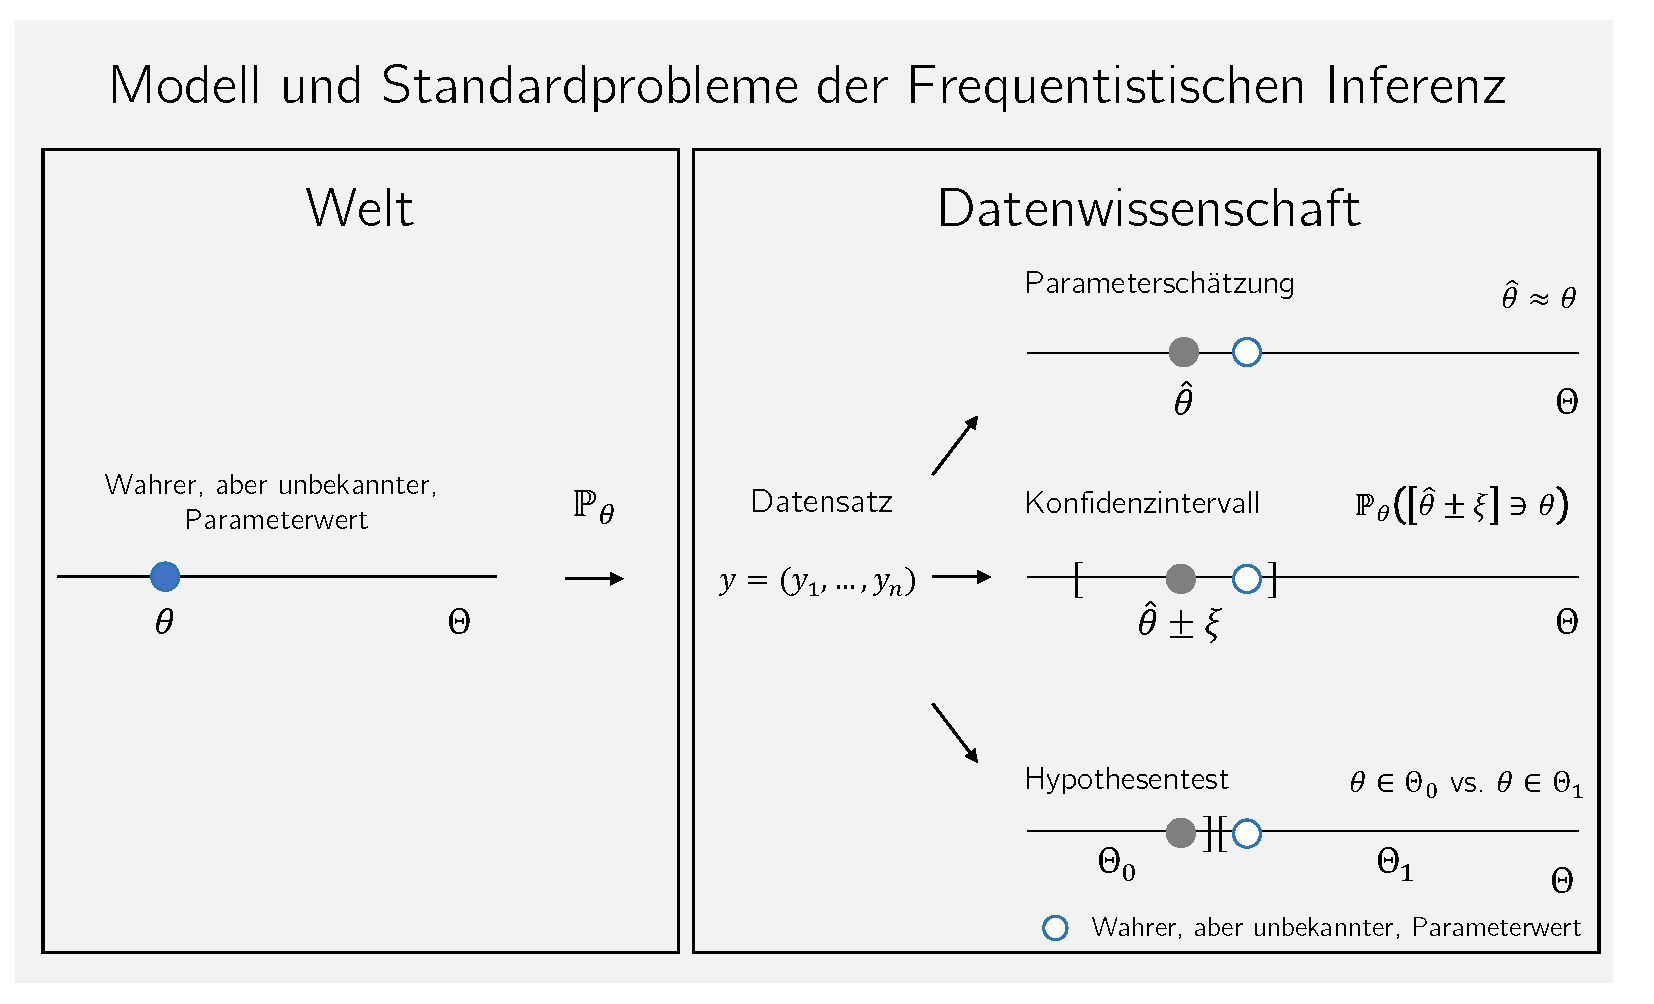
\includegraphics[width=1\linewidth]{6_Abbildungen/alm_6_frequentistische_inferenz} \end{center}
\end{frame}

\begin{frame}{Überblick}
\protect\hypertarget{uxfcberblick-4}{}
\small

Standardannahmen frequentistischer Inferenz

\footnotesize
\setstretch{1.2}

Gegeben sei ein statistisches Modell mit. Es wird angenommen, dass ein
vorliegender Datensatz eine der möglichen Realisierungen der Daten des
Modells ist. Aus frequentistischer Sicht kann man unendlich oft
Datensätze basierend auf einem Modell generieren und zu jedem Datensatz
Schätzer oder Statistiken auswerten, z.B. den Betaparameterschätzer
\vspace{1mm}

\begin{itemize}
\item[] Datensatz (1) : $y^{(1)} = \left(y_1^{(1)}, y_2^{(1)}, ...,y_n^{(1)}\right)^T$  mit $\hat{\beta}^{(1)} = (X^TX)^{-1}X^Ty^{(1)}$
\item[] Datensatz (2) : $y^{(2)} = \left(y_1^{(2)}, y_2^{(2)}, ...,y_n^{(2)}\right)^T$  mit $\hat{\beta}^{(2)} = (X^TX)^{-1}X^Ty^{(2)}$
\item[] Datensatz (3) : $y^{(3)} = \left(y_1^{(3)}, y_2^{(3)}, ...,y_n^{(3)}\right)^T$  mit $\hat{\beta}^{(3)} = (X^TX)^{-1}X^Ty^{(3)}$
\item[] Datensatz (4) : $y^{(4)} = \left(y_1^{(4)}, y_2^{(4)}, ...,y_n^{(4)}\right)^T$  mit $\hat{\beta}^{(4)} = (X^TX)^{-1}X^Ty^{(4)}$
\item[] Datensatz (5) : $y^{(5)} = ...$
\end{itemize}

\vspace{1mm}

Um die Qualität statistischer Methoden zu beurteilen betrachtet die
frequentistische Statistik die Wahrscheinlichkeitsverteilungen von
Schätzern und Statistiken unter Annahme der Datenverteilung. Was zum
Beispiel ist die Verteilung von \(\hat{\beta}^{(1)}\),
\(\hat{\beta}^{(2)}\), \(\hat{\beta}^{(3)}\), \(\hat{\beta}^{(4)}\),
\ldots{} also die Verteilung der Zufallsvariable
\(\hat{\beta} := (X^TX)^{-1}X^Ty\)? Wenn eine statistische Methode im
Sinne der frequentitischen Standardannahmen ``gut'' ist, dann heißt das
also, dass sie bei häufiger Anwendung ``im Mittel gut'' ist. Im
Einzelfall, also im Normalfall nur eines vorliegenden Datensatzes, kann
sie auch ``schlecht'' sein.
\end{frame}

\begin{frame}{}
\protect\hypertarget{section-2}{}
\large
\setstretch{3}
\vfill

Allgemeine Theorie

Unabhängige und identisch normalverteilte Zufallsvariablen

Einfache lineare Regression

Selbstkontrollfragen \vfill
\end{frame}

\begin{frame}{}
\protect\hypertarget{section-3}{}
\large
\setstretch{3}
\vfill

\textbf{Allgemeine Theorie}

Unabhängige und identisch normalverteilte Zufallsvariablen

Einfache lineare Regression

Selbstkontrollfragen

\vfill
\end{frame}

\begin{frame}{Allgemeine Theorie}
\protect\hypertarget{allgemeine-theorie}{}
\footnotesize
\begin{theorem}[Betaparameterschätzer]
\justifying
\normalfont
Es sei
\begin{equation}
y = X\beta + \varepsilon \mbox{ mit } \varepsilon \sim N(0_n,\sigma^2I_n)
\end{equation}
das ALM in generativer Form und es sei
\begin{equation}
\hat{\beta} := (X^TX)^{-1}X^Ty.
\end{equation}
der \textit{Betaparameterschätzer}. Dann gilt für festes $y \in \mathbb{R}^n$, dass
\begin{equation}
\hat{\beta} = \argmin_{\tilde{\beta}} (y - X\tilde{\beta})^T(y - X\tilde{\beta})
\end{equation}
und dass $\hat{\beta}$ ein unverzerrter Maximum Likelihood Schätzer von $\beta \in \mathbb{R}^p$ ist.
\end{theorem}

Bemerkungen

\begin{itemize}
\tightlist
\item
  Das Theorem gibt ein Formel an, um \(\beta\) anhand von Designmatrix
  und Daten zu schätzen.
\item
  Als ML Schätzer ist \(\hat{\beta}\) konsistent, asymptotisch
  normalverteilt und asymptotisch effizient.
\item
  Wir sehen später, dass \(\hat{\beta}\) sogar normalverteilt ist.
\item
  Außerdem hat \(\hat{\beta}\) die ``kleinste Varianz'' in der Klasse
  der linearen unverzerrten Schätzer von \(\beta\).
\item
  Letztere Eigenschaft ist Kernaussage des
  \textit{Gauss-Markov Theorems}, auf das wir hier nicht näher eingehen
  wollen.
\item
  Für eine Diskussion und einen Beweis des Gauss-Markov Theorems siehe
  z.B. Searle (1971), Kapitel 3.
\end{itemize}
\end{frame}

\begin{frame}{Allgemeine Theorie}
\protect\hypertarget{allgemeine-theorie-1}{}
\footnotesize

\underline{Beweis}

\noindent (1) Wir zeigen in einem ersten Schritt, dass \(\hat{\beta}\)
die Summe der Abweichungsquadrate \begin{equation}
(y - X\tilde{\beta})^T(y - X\tilde{\beta})
\end{equation} minimiert. Dazu halten wir zunächst fest, dass
\begin{equation}
\hat{\beta} = (X^TX)^{-1}X^Ty 
\Leftrightarrow 
X^TX\hat{\beta} = X^Ty
\Leftrightarrow 
X^Ty - X^TX\hat{\beta} = 0_p
\Leftrightarrow 
X^T(y -  X\hat{\beta}) = 0_p.
\end{equation} Weiterhin gilt dann auch, dass \begin{equation}
X^T(y - X\hat{\beta}) = 0_p
\Leftrightarrow
\left(X^T(y - X\hat{\beta})\right)^T = 0_p^T
\Leftrightarrow
(y - X\hat{\beta})^TX = 0_p^T
\end{equation} Weiterhin halten wir ohne Beweis fest, dass für jede
Matrix \(X \in \mathbb{R}^{n \times p}\) gilt, dass \begin{equation}
z^TX^TXz \ge 0 \mbox{ für alle } z \in \mathbb{R}^p.
\end{equation} Wir betrachten nun für festes \(y\) und ein beliebiges
\(\tilde{\beta}\) die Summe der Abweichungsquadrate \begin{equation}
(y - X\tilde{\beta})^T(y - X\tilde{\beta}).
\end{equation}
\end{frame}

\begin{frame}{Allgemeine Theorie}
\protect\hypertarget{allgemeine-theorie-2}{}
\footnotesize

\underline{Beweis (fortgeführt)}

Es ergibt sich \begin{align}
\begin{split}
(y - X\tilde{\beta})^T(y - X\tilde{\beta})
& = (y - X\hat{\beta} + X\hat{\beta} - X\tilde{\beta})^T(y - X\hat{\beta} + X\hat{\beta} - X\tilde{\beta}) \\
& = ((y - X\hat{\beta}) + X(\hat{\beta} -\tilde{\beta}))^T((y - X\hat{\beta}) + X(\hat{\beta} -\tilde{\beta})) \\
& = \quad\quad
     (y - X\hat{\beta})^T(y - X\hat{\beta})
   + (y - X\hat{\beta})^T X(\hat{\beta} -\tilde{\beta}) \\
&  \quad\quad
   + (\hat{\beta} -\tilde{\beta})^TX^T(y - X\hat{\beta})
   + (\hat{\beta} -\tilde{\beta})^TX^TX(\hat{\beta} -\tilde{\beta}) \\
& = \quad\quad
     (y - X\hat{\beta})^T(y - X\hat{\beta})
   +  0_p^T(\hat{\beta} -\tilde{\beta}) \\
&  \quad\quad
   + (\hat{\beta} -\tilde{\beta})^T0_p
   + (\hat{\beta} -\tilde{\beta})^TX^TX(\hat{\beta} -\tilde{\beta}) \\
& = (y - X\hat{\beta})^T(y - X\hat{\beta}) + (\hat{\beta} -\tilde{\beta})^TX^TX(\hat{\beta} -\tilde{\beta}) \\
\end{split}
\end{align} Auf der rechten Seite obiger Gleichung ist nur der zweite
Term von \(\tilde{\beta}\) abhängig. Da für diesen Term weiterhin gilt,
dass \begin{equation}
(\hat{\beta} -\tilde{\beta})^TX^TX(\hat{\beta} -\tilde{\beta}) \ge 0
\end{equation} nimmt dieser Term genau dann seinen Minimalwert 0 an,
wenn \begin{equation}
(\hat{\beta} -\tilde{\beta}) = 0_p \Leftrightarrow \tilde{\beta} = \hat{\beta}.
\end{equation} Also gilt \begin{equation}
\hat{\beta} = \argmin_{\tilde{\beta}} (y - X\tilde{\beta})^T(y - X\tilde{\beta}).
\end{equation}
\end{frame}

\begin{frame}{Allgemeine Theorie}
\protect\hypertarget{allgemeine-theorie-3}{}
\footnotesize

\underline{Beweis (fortgeführt)}

\noindent (2) Um zu zeigen, dass \(\hat{\beta}\) ein Maximum Likelihood
Schätzer ist, betrachten wir für festes \(y \in \mathbb{R}^n\) und
festes \(\sigma^2 > 0\) die Log-Likelihood Funktion \begin{equation}
\ell : \mathbb{R}^p \to \mathbb{R}_{>0}, \tilde{\beta} \mapsto \ln p_{\tilde{\beta}}(y) = \ln N(y;X\tilde{\beta}, \sigma^2I_n)
\end{equation} wobei gilt, dass \begin{align}
\begin{split}
\ln N(y;X\tilde{\beta}, \sigma^2I_n)
& = \ln\left((2\pi)^{-\frac{n}{2}}|\sigma^2I_n|^{-\frac{1}{2}}\exp\left(-\frac{1}{2\sigma^2}(y - X\tilde{\beta})^T(y - X\tilde{\beta})\right)\right) \\
& = -\frac{n}{2} \ln 2\pi - \frac{1}{2} \ln |\sigma^2I_n| - \frac{1}{2\sigma^2}(y - X\tilde{\beta})^T(y - X\tilde{\beta})
\end{split}
\end{align} Dabei hängt allein der Term \begin{equation}
- \frac{1}{2\sigma^2}(y - X\tilde{\beta})^T(y - X\tilde{\beta})
\end{equation} von \(\tilde{\beta}\) ab und wird aufgrund des
Vorzeichens maximal, wenn der Term \begin{equation}
(y - X\tilde{\beta})^T(y - X\tilde{\beta})
\end{equation} minimal wird. Dies ist aber wie oben gezeigt genau für
\begin{equation}
\tilde{\beta} = \hat{\beta}
\end{equation} der Fall.
\end{frame}

\begin{frame}{Allgemeine Theorie}
\protect\hypertarget{allgemeine-theorie-4}{}
\footnotesize

\underline{Beweis (fortgeführt)}

\noindent (3) Die Unverzerrtheit von \(\hat{\beta}\) schließlich ergibt
sich aus \begin{align}
\begin{split}
\mathbb{E}(\hat{\beta}) 
= \mathbb{E}\left((X^TX)^{-1}X^Ty\right) 
= (X^TX)^{-1}X^T\mathbb{E}(y) 
= (X^TX)^{-1}X^TX\beta 
= \beta.
\end{split}
\end{align}
\end{frame}

\begin{frame}{Allgemeine Theorie}
\protect\hypertarget{allgemeine-theorie-5}{}
\small
\begin{theorem}[Varianzparameterschätzer]
\justifying
\normalfont
Es sei 
\begin{equation}
y = X\beta + \varepsilon \mbox{ mit } \varepsilon \sim N(0_n,\sigma^2I_n)
\end{equation}
das ALM in generativer Form. Dann ist
\begin{equation}
\hat{\sigma}^2 := \frac{(y - X\hat{\beta})^T(y - X\hat{\beta})}{n - p}
\end{equation}
ein unverzerrter Schätzer von $\sigma^2 > 0$.
\end{theorem}

\footnotesize

Bemerkungen

\begin{itemize}
\tightlist
\item
  Es handelt sich bei \(\hat{\sigma}^2\) \textit{nicht} um einen ML
  Schätzer von \(\sigma^2\).
\item
  Für einen Beweis siehe z.B. Searle (1971), Kapitel 3 oder Rencher and
  Schaalje (2008), Kapitel 7.
\end{itemize}
\end{frame}

\begin{frame}{}
\protect\hypertarget{section-4}{}
\large
\setstretch{3}
\vfill

Allgemeine Theorie

\textbf{Unabhängige und identisch normalverteilte Zufallsvariablen}

Einfache lineare Regression

Selbstkontrollfragen \vfill
\end{frame}

\begin{frame}{Unabhängige und identisch normalverteilte
Zufallsvariablen}
\protect\hypertarget{unabhuxe4ngige-und-identisch-normalverteilte-zufallsvariablen}{}
\footnotesize

Wir betrachten das Szenario von \(n\) Unabhängige und identisch
normalverteilte Zufallsvariablen mit Erwartungswertparameter
\(\mu \in \mathbb{R}\) und Varianzparameter \(\sigma^2\),
\begin{equation}
y_i \sim N(\mu,\sigma^2) \mbox{ für } i = 1,...,n.
\end{equation} Dann gilt, wie unten gezeigt,
\begin{equation}\label{eq:iid_estimators}
\hat{\beta} = \frac{1}{n}\sum_{i=1}^n y_i =: \bar{y}
\mbox{ und }
\hat{\sigma}^2 = \frac{1}{n-1}\sum_{i=1}^n (y_i - \bar{y})^2 =: s^2_y.
\end{equation} In diesem Fall ist also der Betaparameterschätzer mit dem
Stichprobenmittel \(\bar{y}\) der \(y_1,...,y_n\) und der
Varianzparameterschätzer mit der Stichprobenvarianz der \(y_1,...,y_n\)
identisch.
\end{frame}

\begin{frame}{Unabhängige und identisch normalverteilte
Zufallsvariablen}
\protect\hypertarget{unabhuxe4ngige-und-identisch-normalverteilte-zufallsvariablen-1}{}
\footnotesize

Für \(\hat{\beta}\) ergibt sich \begin{align*}
\begin{split}
\hat{\beta}
& = (X^TX)^{-1}X^T y
\\
& =
\left(
\begin{pmatrix}
1 & \cdots & 1\\
\end{pmatrix}
\begin{pmatrix}
1\\
\vdots \\
1\\
\end{pmatrix}
\right)^{-1}
\begin{pmatrix}
1 & \cdots & 1\\
\end{pmatrix}
\begin{pmatrix}
y_{1}\\
\vdots \\
y_{n}\\
\end{pmatrix}
\\
& = n^{-1}\sum_{i=1}^n y_i
\\
& =\frac{1}{n}\sum_{i=1}^n y_i
\\
& =: \bar{y}.
\end{split}
\end{align*}
\end{frame}

\begin{frame}{Unabhängige und identisch normalverteilte
Zufallsvariablen}
\protect\hypertarget{unabhuxe4ngige-und-identisch-normalverteilte-zufallsvariablen-2}{}
\footnotesize

Für \(\hat{\sigma}^2\) ergibt sich \begin{align*}
\begin{split}
\hat{\sigma}^2
& = \frac{1}{n-1}\left(y-X\hat{\beta}\right)^T\left(y-X\hat{\beta} \right)
\\
& = \frac{1}{n-1}
\left(
\begin{pmatrix} y_1 \\  \vdots  \\  y_n \\  \end{pmatrix} -
\begin{pmatrix} 1       \\  \vdots  \\  1     \\    \end{pmatrix}
\left(\frac{1}{n}\sum_{i=1}^n y_i \right)
\right)^T
\left(
\begin{pmatrix} y_1 \\  \vdots  \\  y_n \\  \end{pmatrix} -
\begin{pmatrix} 1       \\  \vdots  \\  1     \\    \end{pmatrix}
\left(\frac{1}{n}\sum_{i=1}^n y_i \right)
\right)
\\
& =
\frac{1}{n-1}
\begin{pmatrix}
y_{1}-\frac{1}{n}\sum_{i=1}^n y_i \\
\vdots \\
y_{n}-\frac{1}{n}\sum_{i=1}^n y_i \\
\end{pmatrix}^T
\begin{pmatrix}
y_{1}-\frac{1}{n}\sum_{i=1}^n y_i \\
\vdots \\
y_{n}-\frac{1}{n}\sum_{i=1}^n y_i \\
\end{pmatrix}
\\
& = \frac{1}{n-1} \sum_{i=1}^n \left(y_i-\frac{1}{n} \sum_{i=1}^n y_i \right)^2
\\
& = \frac{1}{n-1}\sum_{i=1}^n \left(y_i-\bar{y} \right)^2
\\
& =: s^2_y.
\end{split}
\end{align*}
\end{frame}

\begin{frame}[fragile]{Unabhängige und identisch normalverteilte
Zufallsvariablen}
\protect\hypertarget{unabhuxe4ngige-und-identisch-normalverteilte-zufallsvariablen-3}{}
\setstretch{1}
\footnotesize

\begin{Shaded}
\begin{Highlighting}[]
\CommentTok{\# Libraries}
\FunctionTok{library}\NormalTok{(MASS)                                    }\CommentTok{\# Multivariate Normalverteilung }

\CommentTok{\# Modellformulierung}
\NormalTok{n         }\OtherTok{=} \DecValTok{12}                                   \CommentTok{\# Anzahl von Datenpunkten}
\NormalTok{p         }\OtherTok{=} \DecValTok{1}                                    \CommentTok{\# Anzahl von Betparametern}
\NormalTok{X         }\OtherTok{=} \FunctionTok{matrix}\NormalTok{(}\FunctionTok{rep}\NormalTok{(}\DecValTok{1}\NormalTok{,n), }\AttributeTok{nrow =}\NormalTok{ n)           }\CommentTok{\# Designmatrix}
\NormalTok{I\_n       }\OtherTok{=} \FunctionTok{diag}\NormalTok{(n)                              }\CommentTok{\# n x n Einheitsmatrix}
\NormalTok{beta      }\OtherTok{=} \DecValTok{2}                                    \CommentTok{\# wahrer, aber unbekannter, Betaparameter}
\NormalTok{sigsqr    }\OtherTok{=} \DecValTok{1}                                    \CommentTok{\# wahrer, aber unbekannter, Varianzparameter}

\CommentTok{\# Datenrealisierung}
\NormalTok{y        }\OtherTok{=}  \FunctionTok{mvrnorm}\NormalTok{(}\DecValTok{1}\NormalTok{, X }\SpecialCharTok{\%*\%}\NormalTok{ beta, sigsqr}\SpecialCharTok{*}\NormalTok{I\_n)   }\CommentTok{\# eine Realisierung eines n{-}dimensionalen ZVs}

\CommentTok{\# Betaparameterschätzung (matlib\textquotesingle{}s inv funktioniert für 1 x 1 Matrizen nicht...)}
\NormalTok{beta\_hat }\OtherTok{=} \FunctionTok{solve}\NormalTok{(}\FunctionTok{t}\NormalTok{(X) }\SpecialCharTok{\%*\%}\NormalTok{ X) }\SpecialCharTok{\%*\%} \FunctionTok{t}\NormalTok{(X) }\SpecialCharTok{\%*\%}\NormalTok{ y      }\CommentTok{\# \textbackslash{}hat\{\textbackslash{}beta\} = (X\^{}T)X\^{}\{{-}1\}X\^{}Ty }

\CommentTok{\# Ausgabe}
\FunctionTok{cat}\NormalTok{(}\StringTok{"beta     : "}\NormalTok{, beta,}
    \StringTok{"}\SpecialCharTok{\textbackslash{}n}\StringTok{hat\{beta\}: "}\NormalTok{, beta\_hat)}
\end{Highlighting}
\end{Shaded}

\begin{verbatim}
> beta     :  2 
> hat{beta}:  1.64
\end{verbatim}
\end{frame}

\begin{frame}[fragile]{Unabhängige und identisch normalverteilte
Zufallsvariablen}
\protect\hypertarget{unabhuxe4ngige-und-identisch-normalverteilte-zufallsvariablen-4}{}
\footnotesize

Simulation der Schätzerunverzerrtheit \vspace{2mm}

\setstretch{1}
\footnotesize

\begin{Shaded}
\begin{Highlighting}[]
\CommentTok{\# Libraries}
\FunctionTok{library}\NormalTok{(MASS)                                      }\CommentTok{\# Multivariate Normalverteilung}

\CommentTok{\# Modellformulierung}
\NormalTok{n        }\OtherTok{=} \DecValTok{12}                                      \CommentTok{\# Anzahl von Datenpunkten}
\NormalTok{p        }\OtherTok{=} \DecValTok{1}                                       \CommentTok{\# Anzahl von Betparametern}
\NormalTok{X        }\OtherTok{=} \FunctionTok{matrix}\NormalTok{(}\FunctionTok{rep}\NormalTok{(}\DecValTok{1}\NormalTok{,n), }\AttributeTok{nrow =}\NormalTok{ n)              }\CommentTok{\# Designmatrix}
\NormalTok{I\_n      }\OtherTok{=} \FunctionTok{diag}\NormalTok{(n)                                 }\CommentTok{\# n x n Einheitsmatrix}
\NormalTok{beta     }\OtherTok{=} \DecValTok{2}                                       \CommentTok{\# wahrer, aber unbekannter, Betaparameter}
\NormalTok{sigsqr   }\OtherTok{=} \DecValTok{1}                                       \CommentTok{\# wahrer, aber unbekannter, Varianzparameter}

\CommentTok{\# Frequentistische Simulation}
\NormalTok{nsim     }\OtherTok{=} \FloatTok{1e5}                                     \CommentTok{\# Anzahl Realisierungen des n{-}dimensionalen ZVs}
\NormalTok{beta\_hat }\OtherTok{=} \FunctionTok{rep}\NormalTok{(}\ConstantTok{NaN}\NormalTok{,nsim)                           }\CommentTok{\# \textbackslash{}hat\{\textbackslash{}beta\} Realisierungsarray}
\ControlFlowTok{for}\NormalTok{(i }\ControlFlowTok{in} \DecValTok{1}\SpecialCharTok{:}\NormalTok{nsim)\{}
\NormalTok{  y           }\OtherTok{=} \FunctionTok{mvrnorm}\NormalTok{(}\DecValTok{1}\NormalTok{, X }\SpecialCharTok{\%*\%}\NormalTok{ beta, sigsqr}\SpecialCharTok{*}\NormalTok{I\_n) }\CommentTok{\# eine Realisierung eines n{-}dimensionalen ZVs}
\NormalTok{  beta\_hat[i] }\OtherTok{=} \FunctionTok{solve}\NormalTok{(}\FunctionTok{t}\NormalTok{(X) }\SpecialCharTok{\%*\%}\NormalTok{ X) }\SpecialCharTok{\%*\%} \FunctionTok{t}\NormalTok{(X) }\SpecialCharTok{\%*\%}\NormalTok{ y   }\CommentTok{\# \textbackslash{}hat\{\textbackslash{}beta\} = (X\^{}T)X\^{}\{{-}1\}X\^{}Ty }
\NormalTok{\}}

\CommentTok{\# Ausgabe}
\FunctionTok{cat}\NormalTok{(}\StringTok{"Wahrer, aber unbekannter, Betaparameter               : "}\NormalTok{, beta,}
    \StringTok{"}\SpecialCharTok{\textbackslash{}n}\StringTok{Geschätzter Erwartungswert des Betaparameterschätzers : "}\NormalTok{, }\FunctionTok{mean}\NormalTok{(beta\_hat))}
\end{Highlighting}
\end{Shaded}

\begin{verbatim}
> Wahrer, aber unbekannter, Betaparameter               :  2 
> Geschätzter Erwartungswert des Betaparameterschätzers :  2
\end{verbatim}
\end{frame}

\begin{frame}{}
\protect\hypertarget{section-5}{}
\large
\setstretch{3}
\vfill

Allgemeine Theorie

Unabhängige und identisch normalverteilte Zufallsvariablen

\textbf{Einfache lineare Regression}

Selbstkontrollfragen \vfill
\end{frame}

\begin{frame}{Einfache lineare Regression}
\protect\hypertarget{einfache-lineare-regression}{}
\footnotesize

Wir betrachten das generative Modell der einfachen linearen Regression
\begin{equation}\label{eq:slr}
y_i = \beta_0 + \beta_1x_i + \varepsilon_i, \varepsilon_i \sim N(0,\sigma^2) \mbox{ für } i = 1,...,n,
\end{equation} Dann gilt \begin{equation}\label{eq:slr_estimators}
\hat{\beta}
= \begin{pmatrix} \hat{\beta}_0 \\ \hat{\beta}_1 \end{pmatrix}
= \begin{pmatrix} \bar{y} - \frac{c_{xy}}{s_x^2}\bar{x} \\ \frac{c_{xy}}{s_x^2} \end{pmatrix}
\mbox{ and }
\hat{\sigma}^2 = \frac{1}{n-2}\sum_{i=1}^n (y_i - (\hat{\beta}_0 + \hat{\beta}_1x_i))^2
\end{equation} wobei \(\bar{x}\) und \(\bar{y}\) die Stichprobenmittel
der \(x_1,...,x_n\) und \(y_1,...,y_n\), respektive, bezeichnen,
\(c_{xy}\) die Stichprobenkovarianz der \(x_1, ...,x_n\) und \(s_x^2\)
die Stichprobenvarianz der \(x_1,...,x_n\) bezeichnen, wie unten
gezeigt.

Wir halten fest, dass für eine parametrische Designmatrixspalte sich der
entsprechende Betaparameterschätzer aus der Stichprobenkovarianz der
respektiven Spalte mit den Daten geteil durch die Stichprobenvarianz der
entsprechenden Spalte ergibt und somit einer ``standardisierten''
Stichhprobenkovarianz entspricht. Wie in (1) Regression sind die
Bezeichnungen ``Stichproben''kovarianz und ``Stichproben''varianz
bezüglich der \(x_1,...,x_n\) hier lediglich formal gemeint, da keine
Annahme zugrundeliegt, dass die \(x_1,...,x_n\) Realisierungen von
Zufallsvariablen sind. Die \(x_1,...,x_n\) sind vorgegebene Werte. Ein
Vergleich mit den Parametern der Ausgleichsgerade in (1) Regression
zeigt weiterhin die Identität der Betaparameterschätzerkomponenten
\(\hat{\beta}_0\) und \(\hat{\beta}_1\) mit den dort unter dem Kriterium
der Minimierung der quadrierten vertikalen Abweichungen hergeleiteten
Parametern. Dies überrascht nicht, da sowohl \(\hat{\beta}\) als auch
die Parameter der Ausgleichsgerade den Wert\\
\begin{equation}
q(\tilde{\beta}) = \sum_{i=1}^n (y_i - (\tilde{\beta}_0 + \tilde{\beta}_1 x_i)) = (y - X\tilde{\beta})^T(y - X\tilde{\beta})
\end{equation} hinsichtlich \(\tilde{\beta}\) minimieren.
\end{frame}

\begin{frame}{Einfache lineare Regression}
\protect\hypertarget{einfache-lineare-regression-1}{}
\footnotesize

Um die Form des Betaparameterschätzers herzuleiten, halten wir zunächst
fest, dass \tiny \begin{align}
\begin{split}
c_{xy}
:= \sum_{i=1}^n (x_i - \bar{x})(y_i - \bar{y})
& = \sum_{i=1}^n (x_iy_i - x_i\bar{y} - \bar{x}y_i + \bar{x}\bar{y}) \\
& = \sum_{i=1}^n x_iy_i
  - \sum_{i=1}^n x_i\bar{y}
  - \sum_{i=1}^n \bar{x}y_i
  + \sum_{i=1}^n \bar{x}\bar{y} \\
& = \sum_{i=1}^n x_iy_i
  - \bar{y} \sum_{i=1}^n x_i
  - \bar{x}\sum_{i=1}^n y_i
  + n \bar{x}\bar{y} \\
& = \sum_{i=1}^n x_iy_i
  - \bar{y}n\bar{x}
  - \bar{x}n\bar{y}
  + n\bar{x}\bar{y} \\
  & = \sum_{i=1}^n x_iy_i
  - n\bar{x}\bar{y}
  - n\bar{x}\bar{y}
  + n\bar{x}\bar{y} \\
& = \sum_{i=1}^n x_i y_i  - n \bar{x}\bar{y},
\end{split}
\end{align}
\end{frame}

\begin{frame}{Einfache lineare Regression}
\protect\hypertarget{einfache-lineare-regression-2}{}
\footnotesize

Weiterhin halten wir fest, dass \tiny \begin{align}
\begin{split}
s_x^2
:= \sum_{i=1}^n (x_i - \bar{x})^2
& = \sum_{i=1}^n (x_i^2 - 2x_i\bar{x}  + \bar{x}^2) \\
& = \sum_{i=1}^n x_i^2 - \sum_{i=1}^n 2x_i\bar{x}  + \sum_{i=1}^n \bar{x}^2 \\
& = \sum_{i=1}^n x_i^2 - 2\bar{x}\sum_{i=1}^n x_i  + n\bar{x}^2 \\
& = \sum_{i=1}^n x_i^2 - 2\bar{x}n\bar{x}  + n\bar{x}^2 \\
& = \sum_{i=1}^n x_i^2 - 2n\bar{x}^2 + n\bar{x}^2 \\
& = \sum_{i=1}^n x_i^2 - n\bar{x}^2.\\
\end{split}
\end{align}
\end{frame}

\begin{frame}{Einfache lineare Regression}
\protect\hypertarget{einfache-lineare-regression-3}{}
\footnotesize

Aus der Definition von \(\hat{\beta}\) ergibt sich \begin{align}
\begin{split}
\hat{\beta}
& = (X^T X)^{-1}X^Ty \\
& =
\left(
\begin{pmatrix}
1   & \cdots & 1 \\
x_1 & \cdots & x_n
\end{pmatrix}
\begin{pmatrix}
1       & x_1       \\
\vdots  & \vdots    \\
1       & x_n
\end{pmatrix}
\right)^{-1}
\begin{pmatrix}
1   & \cdots & 1 \\
x_1 & \cdots & x_n
\end{pmatrix}
\begin{pmatrix}
y_1     \\
\vdots  \\
y_n
\end{pmatrix} \\
& =
\begin{pmatrix}
n                   & \sum_{i=1}^n x_i \\
\sum_{i=1}^n x_i    & \sum_{i=1}^n x_i^2\\
\end{pmatrix}^{-1}
\begin{pmatrix}
\sum_{i=1}^n y_i    \\
\sum_{i=1}^n x_i y_i    \\
\end{pmatrix}
\\
& =
\begin{pmatrix}
n           &  n\bar{x} \\
n\bar{x}    & \sum_{i=1}^n x_i^2\\
\end{pmatrix}^{-1}
\begin{pmatrix}
n\bar{y}    \\
\sum_{i=1}^n x_i y_i    \\
\end{pmatrix}.
\end{split}
\end{align}

Die Inverse von \(X^T X\) ist gegeben durch \begin{equation}
\frac{1}{s_x^2}
\begin{pmatrix}
  \frac{s_x^2}{n} + \bar{x}^2
& -\bar{x}
\\
  -\bar{x}
&  1
\end{pmatrix},
\end{equation}
\end{frame}

\begin{frame}{Einfache lineare Regression}
\protect\hypertarget{einfache-lineare-regression-4}{}
\footnotesize

weil \begin{align}
\begin{split}
& \frac{1}{s_x^2}
\begin{pmatrix}
  \frac{s_x^2}{n} + \bar{x}^2
& -\bar{x}
\\
  -\bar{x}
&  1
\end{pmatrix}
\begin{pmatrix}
n           &  n\bar{x} \\
n\bar{x}    & \sum_{i=1}^n x_i^2\\
\end{pmatrix}
\\
& =
\frac{1}{s_x^2}
\begin{pmatrix}
\frac{ns_x^2}{n} + n\bar{x}^2 - n \bar{x}^2
& \frac{s_x^2n\bar{x}}{n} +n\bar{x}^2\bar{x} - \bar{x}\sum_{i=1}^n x_i^2
\\
-\bar{x}n + n \bar{x}
& - n\bar{x}^2 + \sum_{i=1}^n x_i^2
\end{pmatrix} \\
& =
\frac{1}{s_x^2}
\begin{pmatrix}
s_x^2
& s_x^2\bar{x} -\bar{x} \left(\sum_{i=1}^n x_i^2 - n\bar{x}^2\right)
\\
0
& \sum_{i=1}^n x_i^2 - n\bar{x}^2
\end{pmatrix}
\\
& =
\frac{1}{s_x^2}
\begin{pmatrix}
s_x^2
& s_x^2\bar{x} - \bar{x} s_x^2
\\
0
& s_x^2
\end{pmatrix}
\\
& =
\frac{1}{s_x^2}
\begin{pmatrix}
s_x^2
& 0
\\
0
& s_x^2
\end{pmatrix}
\\
& =
\begin{pmatrix}
1 & 0 \\ 0 & 1
\end{pmatrix}.
\end{split}
\end{align}
\end{frame}

\begin{frame}{Einfache lineare Regression}
\protect\hypertarget{einfache-lineare-regression-5}{}
\footnotesize

Es ergibt sich also \begin{align}
\renewcommand{\arraystretch}{1.2}
\begin{split}
\hat{\beta}
= \begin{pmatrix}
  \frac{1}{n} + \frac{\bar{x}^2}{s_x^2}
& -\frac{\bar{x}}{s_x^2}
\\
  -\frac{\bar{x}}{s_x^2}
&  \frac{1}{s_x^2}
\end{pmatrix}
\begin{pmatrix}
n\bar{y}    \\
\sum_{i=1}^n x_i y_i    \\
\end{pmatrix}
& = \begin{pmatrix}
\left(\frac{1}{n} + \frac{\bar{x}^2}{s_x^2}\right)n\bar{y} - \frac{\bar{x}\sum_{i=1}^n x_iy_i}{s_x^2}   \\
\frac{\sum_{i=1}^n x_i y_i }{s_x^2} - \frac{n\bar{x}\bar{y}}{s_x^2} \\
\end{pmatrix}
\\
&
=
\begin{pmatrix}
\frac{n\bar{y}}{n} + \frac{\bar{x}^2n\bar{y}}{s_x^2}- \frac{\bar{x}\sum_{i=1}^n x_iy_i}{s_x^2}
\\
\frac{\sum_{i=1}^n x_i y_i - n\bar{x}\bar{y}}{s_x^2}    \\
\end{pmatrix}
\\
& =
\begin{pmatrix}
\bar{y} + \frac{\bar{x}n\bar{x}\bar{y} - \bar{x}\sum_{i=1}^n x_iy_i}{s_x^2}
\\
\frac{\sum_{i=1}^n x_i y_i - n\bar{x}\bar{y}}{s_x^2}    \\
\end{pmatrix}
\\
& =
\begin{pmatrix}
\bar{y} - \frac{\sum_{i=1}^n x_iy_i - n\bar{x}\bar{y}}{s_x^2}\bar{x}
\\
\frac{\sum_{i=1}^n x_i y_i - n\bar{x}\bar{y}}{s_x^2}
\end{pmatrix}
\\
& =
\begin{pmatrix}
\bar{y} - \frac{c_{xy}}{s_x^2}\bar{x}
\\
\frac{c_{xy}}{s_x^2}
\end{pmatrix}.
\end{split}
\end{align}
\end{frame}

\begin{frame}[fragile]{Einfache lineare Regression}
\protect\hypertarget{einfache-lineare-regression-6}{}
\setstretch{1}
\footnotesize

\begin{Shaded}
\begin{Highlighting}[]
\CommentTok{\# Libraries}
\FunctionTok{library}\NormalTok{(MASS)                                  }\CommentTok{\# Multivariate Normalverteilung }
\FunctionTok{library}\NormalTok{(matlib)                                }\CommentTok{\# Matrizenrechnung}

\CommentTok{\# Modellformulierung}
\NormalTok{n        }\OtherTok{=} \DecValTok{10}                                  \CommentTok{\# Anzahl von Datenpunkten}
\NormalTok{p        }\OtherTok{=} \DecValTok{2}                                   \CommentTok{\# Anzahl von Betaparametern}
\NormalTok{x        }\OtherTok{=} \DecValTok{1}\SpecialCharTok{:}\NormalTok{n                                 }\CommentTok{\# Prädiktorwerte}
\NormalTok{X        }\OtherTok{=} \FunctionTok{matrix}\NormalTok{(}\FunctionTok{c}\NormalTok{(}\FunctionTok{rep}\NormalTok{(}\DecValTok{1}\NormalTok{,n),x), }\AttributeTok{nrow =}\NormalTok{ n)     }\CommentTok{\# Designmatrix}
\NormalTok{I\_n      }\OtherTok{=} \FunctionTok{diag}\NormalTok{(n)                             }\CommentTok{\# n x n Einheitsmatrix}
\NormalTok{beta     }\OtherTok{=} \FunctionTok{matrix}\NormalTok{(}\FunctionTok{c}\NormalTok{(}\DecValTok{0}\NormalTok{,}\DecValTok{1}\NormalTok{), }\AttributeTok{nrow =}\NormalTok{ p)            }\CommentTok{\# wahrer, aber unbekannter, Betaparameter}
\NormalTok{sigsqr   }\OtherTok{=} \DecValTok{1}                                   \CommentTok{\# wahrer, aber unbekannter, Varianzparameter}

\CommentTok{\# Datenrealisierung}
\NormalTok{y        }\OtherTok{=} \FunctionTok{mvrnorm}\NormalTok{(}\DecValTok{1}\NormalTok{, X }\SpecialCharTok{\%*\%}\NormalTok{ beta, sigsqr}\SpecialCharTok{*}\NormalTok{I\_n)  }\CommentTok{\# eine Realisierung eines n{-}dimensionalen ZVs}
\NormalTok{beta\_hat }\OtherTok{=} \FunctionTok{inv}\NormalTok{(}\FunctionTok{t}\NormalTok{(X) }\SpecialCharTok{\%*\%}\NormalTok{ X) }\SpecialCharTok{\%*\%} \FunctionTok{t}\NormalTok{(X) }\SpecialCharTok{\%*\%}\NormalTok{ y      }\CommentTok{\# \textbackslash{}hat\{\textbackslash{}beta\} = (X\^{}TX)\^{}\{{-}1\}X\^{}Ty}

\CommentTok{\# Ausgabe}
\FunctionTok{cat}\NormalTok{(}\StringTok{"beta     : "}\NormalTok{  , beta,}
    \StringTok{"}\SpecialCharTok{\textbackslash{}n}\StringTok{hat\{beta\}: "}\NormalTok{, beta\_hat)}
\end{Highlighting}
\end{Shaded}

\begin{verbatim}
> beta     :  0 1 
> hat{beta}:  -0.265 0.966
\end{verbatim}
\end{frame}

\begin{frame}[fragile]{Unabhängige und identisch normalverteilte
Zufallsvariablen}
\protect\hypertarget{unabhuxe4ngige-und-identisch-normalverteilte-zufallsvariablen-5}{}
\footnotesize

Simulation der Schätzerunverzerrtheit \vspace{2mm}

\setstretch{1}
\footnotesize

\begin{Shaded}
\begin{Highlighting}[]
\CommentTok{\# Libraries}
\FunctionTok{library}\NormalTok{(MASS)                                       }\CommentTok{\# Multivariate Normalverteilung }
\FunctionTok{library}\NormalTok{(matlib)                                     }\CommentTok{\# Matrizenrechnung}

\CommentTok{\# Modellformulierung}
\NormalTok{n        }\OtherTok{=} \DecValTok{10}                                       \CommentTok{\# Anzahl von Datenpunkten}
\NormalTok{p        }\OtherTok{=} \DecValTok{2}                                        \CommentTok{\# Anzahl von Betparametern}
\NormalTok{x        }\OtherTok{=} \DecValTok{1}\SpecialCharTok{:}\NormalTok{n                                      }\CommentTok{\# Prädiktorwerte}
\NormalTok{X        }\OtherTok{=} \FunctionTok{matrix}\NormalTok{(}\FunctionTok{c}\NormalTok{(}\FunctionTok{rep}\NormalTok{(}\DecValTok{1}\NormalTok{,n),x), }\AttributeTok{nrow =}\NormalTok{ n)          }\CommentTok{\# Designmatrix}
\NormalTok{I\_n      }\OtherTok{=} \FunctionTok{diag}\NormalTok{(n)                                  }\CommentTok{\# n x n Einheitsmatrix}
\NormalTok{beta     }\OtherTok{=} \FunctionTok{matrix}\NormalTok{(}\FunctionTok{c}\NormalTok{(}\DecValTok{0}\NormalTok{,}\DecValTok{1}\NormalTok{), }\AttributeTok{nrow =}\NormalTok{ p)                 }\CommentTok{\# wahrer, aber unbekannter, Betaparameter}
\NormalTok{sigsqr   }\OtherTok{=} \DecValTok{1}                                        \CommentTok{\# wahrer, aber unbekannter, Varianzparameter}

\CommentTok{\# Frequentistische Simulation}
\NormalTok{nsim     }\OtherTok{=} \FloatTok{1e4}                                      \CommentTok{\# Anzahl Realisierungen des n{-}dimensionalen ZVs}
\NormalTok{beta\_hat }\OtherTok{=} \FunctionTok{matrix}\NormalTok{(}\FunctionTok{rep}\NormalTok{(}\ConstantTok{NaN}\NormalTok{,p}\SpecialCharTok{*}\NormalTok{nsim), }\AttributeTok{nrow =}\NormalTok{ p)        }\CommentTok{\# \textbackslash{}hat\{\textbackslash{}beta\} Realisierungsarray}
\ControlFlowTok{for}\NormalTok{(i }\ControlFlowTok{in} \DecValTok{1}\SpecialCharTok{:}\NormalTok{nsim)\{}
\NormalTok{  y            }\OtherTok{=} \FunctionTok{mvrnorm}\NormalTok{(}\DecValTok{1}\NormalTok{, X }\SpecialCharTok{\%*\%}\NormalTok{ beta, sigsqr}\SpecialCharTok{*}\NormalTok{I\_n) }\CommentTok{\# eine Realisierung eines n{-}dimensionalen ZVs}
\NormalTok{  beta\_hat[,i] }\OtherTok{=} \FunctionTok{inv}\NormalTok{(}\FunctionTok{t}\NormalTok{(X) }\SpecialCharTok{\%*\%}\NormalTok{ X) }\SpecialCharTok{\%*\%} \FunctionTok{t}\NormalTok{(X) }\SpecialCharTok{\%*\%}\NormalTok{ y     }\CommentTok{\# \textbackslash{}hat\{\textbackslash{}beta\} = (X\^{}T)X\^{}\{{-}1\}X\^{}Ty }
\NormalTok{\}}

\CommentTok{\# Ausgabe}
\FunctionTok{cat}\NormalTok{(}\StringTok{"Wahrer, aber unbekannter, Betaparameter               : "}\NormalTok{, beta,}
    \StringTok{"}\SpecialCharTok{\textbackslash{}n}\StringTok{Geschätzter Erwartungswert des Betaparameterschätzers : "}\NormalTok{, }\FunctionTok{rowMeans}\NormalTok{(beta\_hat))}
\end{Highlighting}
\end{Shaded}

\begin{verbatim}
> Wahrer, aber unbekannter, Betaparameter               :  0 1 
> Geschätzter Erwartungswert des Betaparameterschätzers :  -0.0016 1
\end{verbatim}
\end{frame}

\begin{frame}{}
\protect\hypertarget{section-6}{}
\large
\setstretch{3}
\vfill

Allgemeine Theorie

Unabhängige und identisch normalverteilte Zufallsvariablen

Einfache lineare Regression

\textbf{Selbstkontrollfragen}

\vfill
\end{frame}

\begin{frame}{Selbstkontrollfragen}
\protect\hypertarget{selbstkontrollfragen}{}
\footnotesize
\setstretch{2}

\begin{enumerate}
\tightlist
\item
  Geben Sie das Betaparameterschätzer Theorem wieder.
\item
  Geben Sie das Varianzparameterschätzer Theorem wieder.
\item
  Geben Sie die Beta- und Varianzparameterschätzer des ALM Szenarios von
  \(n\) unabhängigen und identisch normalverteilten Zufallsvariablen
  wieder.
\item
  Geben Sie die Beta- und Varianzparameterschätzer des ALM Szenarios der
  einfachen linearen Regression wieder.
\item
  Wie unterscheiden sich die Betaparameterschätzer des ALM Szenarios der
  einfachen linearen Regression und die Parameter der Ausgleichsgerade
  aus Einheit (1) Regression?
\item
  Simulieren Sie die Unverzerrtheit des Varianzparameterschätzers im ALM
  Szenario von von \(n\) unabhängigen und identisch normalverteilten
  Zufallsvariablen in einem R Skript.
\item
  Simulieren Sie die Unverzerrtheit des Varianzparameterschätzers im ALM
  Szenario der einfachen linearen Regression in einem R Skript.
\end{enumerate}
\end{frame}

\begin{frame}{References}
\protect\hypertarget{references}{}
\footnotesize

\hypertarget{refs}{}
\begin{CSLReferences}{1}{0}
\leavevmode\vadjust pre{\hypertarget{ref-rencher_2008}{}}%
Rencher, Alvin C., and G. Bruce Schaalje. 2008. \emph{Linear Models in
Statistics}. 2nd ed. {Hoboken, N.J}: {Wiley-Interscience}.

\leavevmode\vadjust pre{\hypertarget{ref-searle_1971}{}}%
Searle, S. R. 1971. \emph{Linear Models}. A {Wiley} Publication in
Mathematical Statistics. {New York}: {Wiley}.

\end{CSLReferences}
\end{frame}

\end{document}
